\begin{figure*}[tb]
\centerline{
\includegraphics[width=2.5in, angle=270 ]{./figures/GrabSeq.eps}
} \caption{An example. Sequence of the robot grasping a porcelain
cup. Frame 1: the cup is presented to the robot. Frame 2: the
robot reaches for the cup. Frames 3 to 6:  the robot explores the
space and uses tactile feedback to find the object and adjust the
position of the hand. Frames 7 and 8: the robot grasps
and lifts the cup.} \label{fig:sequence}
\end{figure*}

\begin{figure*}[tb]
  \centerline{
    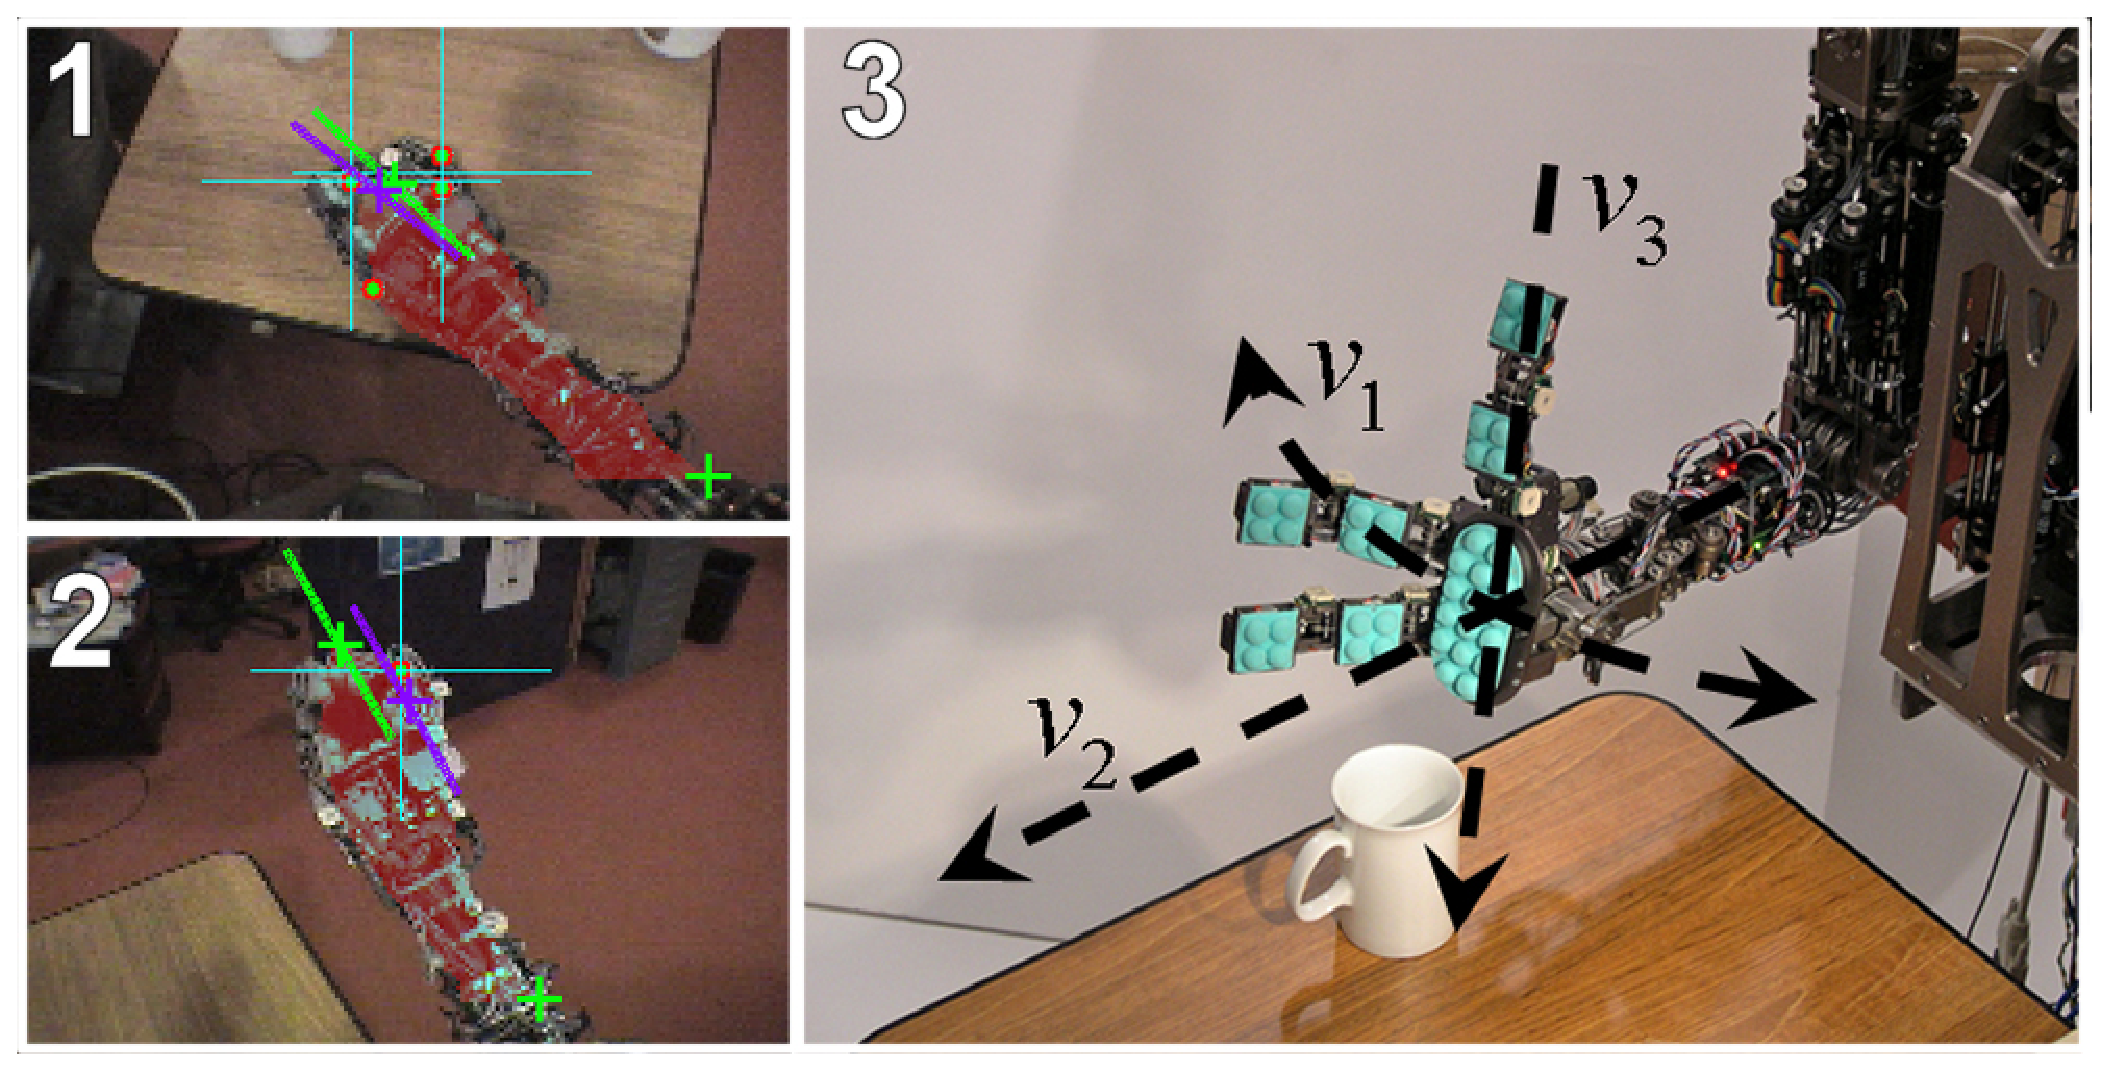
\includegraphics[width=2.5in, angle=0 ]{./figures/expl-directions.eps}
  }\caption{Left, frames 1 and 2: hand localization and arm 
    orientation. Right, frame 3: exploration primitives. Primitives $v_1$ 
and $v_3$ are perpendicular and parallel to the arm orientation. $v_2$ is 
along the null space of the arm Jacobian. See section~\cite{sec:controlling} for
 more details.}
\label{fig:expl-directions}
\end{figure*}

\section{Controlling the body}
\label{sec:controlling}

In this section we describe a few perceptual and motor competencies required 
for the robot to be able to control the body in a meaningful and safe way: 
this includes a simple attention system to spot the objects to be grasped 
and the ability to control the body to reach out for them. A the end of the
section we describe how the these capabilities are integrated in the grasping 
behavior.

\subsection{Attention System}
Motion is a simple yet powerful cue to select points of interest in the visual
scene; for an active camera system this is still true assuming we can estimate 
the motion of the background and account for it. In this paper we use the 
algorithm proposed by \cite{kemp-thesis}, which uses a 2D affine model to 
robustly estimate the image motion resulting from the background. In short the 
algorithm measures the motion of each pixel with a block matching procedure, and 
performs a least square fitting of the global affine model. Using the affine model
the algorithm performs a prediction of the motion of each edge, and marks as 
foreground those edges that poorly match this prediction. Under the assumption 
that the mojority of the image motion relate to the background, these edges 
can be used to build a saliency map to direct the attention of the robot. 

\subsection{Eye-hand coordination}
Given the topic of our research, we decided to focus on explorative 
actions rather than precise, goal directed, actions towards the target objects.
This was also motivated by the fact that the monocular visual system of Obrero
makes depth estimation very difficult. This situation is actually quite common 
in robotics, as depth estimation in real time is a challenging problem even with 
stereo vision.
On the other hand, however, we cannot hope to program the robot to perform 
a blind exploration of the entire workspace. A possible solution is to 
constran the exploration to the area of the workspace where the object is 
detected visually. Since the 3D location of the object is not available reaching 
is performed in 2D; the exploration procedure allows the robot to find the actual
position of the object. The motor skills required for reaching and performing 
the exploration can be learnt starting from the visual abilities 
to localize the hand and compute the orientation of the arm.

\subsection{Hand Localization}
A visual module detects the hand and computes the orientation of 
the arm in the image. The initial step of the arm detector consists
in running a high frequency filter. All points whose frequency 
is below a certain threshold (fixed a priori) are discarded. 
A blob detector is run on the resulting image and the biggest blob
is selected as the arm. The orientation of the arm is computed as the 
orientation of the line passing through the top-most and bottom-most 
pixels of the arm area.
Next, specific features (the small circular black and white 
potentiometers on the fingers) are searched on the arm
area. The hand is identified if more than three of these features are
found.
The detection just desribed proved reliable enough for our purposes 
and was used as a short-cut in place of other, more general, 
methods \cite{metta03early,natale05from}.

The visual feedback of the hand could be used for closed-loop control. 
However closed-loop control is not always suitable. This happens for example 
in presence of occlusions or when the hand is not within the visual field. 

Open-loop control is an alternative solution. A possible open-loop control 
consits in a mapping between the fixation point of the head and the arm 
end-point \cite{metta00Babybot}. The advantage of this approach is that the mapping 
can be easily learnt if the robot can fixate the hand. Another approch is to
use the hand localization to learn a direct mapping between the arm 
proprioception (encoder feedback) and the position of the arm in the visual 
space \cite{natale05from}. The direct (forward) mapping can be inverted 
locally to control the arm to reach for a visually identified target. The 
solution we adopt here is similar: in a discovery phase the robot
tracks the hand as the arm moves to randomly explore the workspace.
This behavior allows the robot to acquires the samples:

\begin{center}
\begin{math}
  \left(\begin{array}{ccccc}
    x & y & \alpha &q_{head} &q_{arm} \end{array}\right)_{0,1\dots,k}
\end{math}
\end{center}

where $x$ and $y$ are the coordinates of the hand in the image,
$\alpha$ is the orientation of the arm, $q_{head}$ and $q_{arm}$ are 
the position of the head and arm respectively. Given $q_{head}$ it is
possible to convert $x$ and $y$ into an egocentric reference frame:
\begin{equation}
  \left(\begin{array}{c}
    \theta \\
    \phi \\
    \end{array}\right)
  = f_{head}^{-1}
  \left(\begin{array}{c}
    x \\
    y \\
    q_{head}
    \end{array} \right)
\label{eq-head-inverse}
\end{equation}

$\theta$ and $\phi$ represents the polar coordinates of the hand in the
reference frame centered at the base of the robot. Basically 
$f_{head}^{-1}$ includes knowledge of the inverse kinematics of the 
head and the parameters of the camera. The opposite transformation maps 
polar coordinates into the image plane:
\begin{equation}
  \left(\begin{array}{c}
    x \\
    y \\
    \end{array}\right)
  = f_{head}
  \left(\begin{array}{c}
    \theta \\
    \phi \\
    q_{head}
    \end{array} \right)
\label{eq-head-direct}
\end{equation}

Given these two transformations a neural newtork can be trained to 
learn the following mapping:

\begin{equation}
  \left(\begin{array}{c}
    \theta \\
    \phi \\
    \alpha \\ 
    \end{array}\right)
  = f \left(q_{arm}\right)
\label{eq-arm-direct}
\end{equation}

which links the arm posture $q_{arm}$ to the polar coordinates of the 
hand $\left(\theta, \phi\right)$ and the orientation of the arm $\alpha$.
To learn this mapping we used a neural netowork suitable for online
learning \cite{schaal98Constructive}.

This mapping allows computing the polar coordinates of the hand with 
respect of the robot from the encoders of the arm. Whenver required 
Equation~\ref{eq-head-direct} maps the polar coordinates back onto 
the image plane.

\subsection{Reaching}
\label{sec:reaching}
Suppose we want to move the arm towards a location of the workspace 
indentified visually. Let $\left(\begin{array}{c} x_t \\ y_t\end{array}\right)$
be such position. Knowing $q_{head}$ from equation \ref{eq-head-inverse} 
we can convert the target position into the body centered reference frame 
$\left(\begin{array}{c} \theta_t  \\ \phi_t\end{array}\right)$. The 
reaching problem can now be stated as a the minimization of the following 
cost funtion:

\begin{equation}
  \displaystyle\min_{q_{arm}}\left(C\right)=\displaystyle\min_{q_{arm}}\left[
  \left(
  \begin{array}{c}
    \theta_t \\
    \phi_t \\
    \end{array}\right)
  -f \left(q_{arm}\right)
  \right]^2
\label{eq-reaching1}
\end{equation}

Assuming a stationary target the minimum of equation \ref{eq-reaching1} 
can be found by gradient descent. The gradient of $C$ is proportional 
to the Jacobian transposed of the manipulator, that is:

\begin{equation}
  \nabla C=-2\nabla f\left(q_{arm}\right)=-2J^T\left(q_{arm}\right)
\label{eq-gradient}
\end{equation}

$\nabla f\left(q_{arm}\right)$ can be approximated by partial 
 differentiation of the mapping of equation \ref{eq-arm-direct}. The 
differentiation can be numerical or analytical (the output of the 
network can be easily differentiated because the basis functions used 
in the neural netowrk are gaussians with known parameters).

To summarize we have described a method to compute the arm commands
required to reach for a visual target. The method employs the 
forwards kinematics of the arm. The direct kinematics is learnt by the 
robot as described in the previous section. The reaching 
problem is solved interatively by using an approximation of the arm
Jacobian. The lattern is obtained by differentiating the basis functions 
of the neural network approximating the direct kinematics. This procedure
is carried out online without using the real visual feedback of the hand.

In the robot visual information (and hence the mapping of equation~\ref{eq-arm-direct}) 
is two-dimensional and does not carry any information
about distance. The solution found by descending the gradient of the 
direct kinematics takes care of minimizing the distance between the target 
and the hand \emph{on the image plane}, and as such, is not concerned 
with the third dimension $R$ (the distance between the hand and the image 
plane, along the optical axis). 
In practice however the components of the gradient along $R$ are small 
compared to the others. The value of $R$ at the end of the reaching movement 
depends on the initial position of the arm; we chose this value so to keep 
the hand above the table.

\subsection{Exploration}
Starting from the direct mapping of the hand position and arm orientation we 
can identify a set of explorative primitives, that is a set of vectors in 
joint space that allows the robot to explore the arm workspace. We chose three 
vectors $v_1$, $v_2$ and $v_3$, as follows:
\begin{equation}
  v_1=k_1J^T\left(\Delta X_1\right)
\end{equation}
where $\Delta X_1$ is vector in the image plane along the direction 
perpendicular to the arm, and $k_1$ is a proportional scale factor;
\begin{equation}
  v_2=k_2J^T\left(\Delta X_2\right)
\end{equation}
where $\Delta X_2$ is vector in the image plane poiting away from the hand 
along the orientation of the arm, and $k_2$ is a proportional scale factor;
\begin{equation}
 v_3\in \ker \left(J\right)
\end{equation}
$v_3$ lays in the null space of the arm Jacobian; in our case the 
null space of the Jacobian consists of those vector that do not affect 
either the projection of the hand onto the visual plane or the orientation 
of the arm. These vectors produce a movement of the hand along the optical 
axis of the camera, or, in other word, along $R$.
$v_1$, $v_2$ and $v_3$ are depicted schematically on the left side of 
Figure~\ref{fig:expl-directions}.

\subsection{A grasping behavior}
In this section we describe the grasping behavior of the robot. The 
sequence begins when the experimenter waves an object in front of the 
robot. The head tracks the object until it remains stationary within 
the workspace of the arm. The robot reaches for the object; motion 
is planned visually as described in section~\ref{sec:reaching}. 
Reaching is not accurate enough to guarantee a correct grasp. Since no 
three dimensional information is available the arm reaches a region 
above the object (see section~\ref{sec:reaching}). At this point the 
exploration starts; the robot computes the explorative 
primitives $v_1$, $v_2$ and $v_3$. The exploration mainly uses three behaviors:

1) \emph{hover behavior}, moves the hand back and forth along $v_1$
2) \emph{push behavior}, moves the hand along $v_2$
3) \emph{depth behavior},  moves the hand ''downwards'' along $v_3$; 
this behavior moves the hand along the direction of the optical axis 
of the camera and adjusts the height of the hand with respect to the 
object/table. To avoid crashing the hand into the table this behavior 
is inhibited when the infrared proximity sensor detects an obstacle 
(usually this happens close to the table).

The \emph{hover behavior} and the \emph{depth behavior} are activated at the 
beginning of the exploration. The goal of this initial phase is to adjust 
the position of the hand until the index finger touches the object. 
This allows adjusting the position of the hand along the directions 
$v_1$ and $v_3$. During the exploration the arm stops when the hand 
detects the object, to avoid pushing it away or knocking it over; if 
no contact is detected, on the other hand, the amplitude of the exploration 
is extended (this increases the probability to touch the object in case 
the reaching error is large); the exploration terminates when 
the contact with the object is detected by any of the tactile sensors 
placed on the index finger.
At this point the \emph{hover behavior} is suspended and the \emph{push behavior} 
activated. The ''pushing'' movement along $v_2$ brings the palm in 
contact with the object while the \emph{depth behavior} takes care of 
maintaining the correct distance with the table. When the robot detects 
contact on the palm the exploration stops and the \emph{grasping behavior} is 
activated. The \emph{grasping behavior} simply closes the fingers to a 
specific position. The low impedance of the joints allows the fingers to 
adapt to the different objects being grasped.

The grasping behavior proved to be quite reliable. Figure \ref{fig:sequence} 
shows an example of the robot grasping a porcelain cup. Repetitive tests 
are described in section~\ref{sec:results}.

% The robot waits for a visual stimula. The robot reaches towards
%the goal without 3D information. If there is not contact detected
%by the tactile sensor, it hover until there is contact.
%Depending on the position of the contact the following actions
%are taken. If touched only on middle finger then the finger
%retracts and keeps hovering to make contact with both fingers.
%If that contact occurs the thumb is opposed to the index finger.
%At this point the robot starts pushing waiting for contact with
%the palm. When the palm sensors are activate the hand is closed
%to grab the object and lift it.

%The behavior of the robot is as follows. It sweeps its hand back
%and forth over a table, and stops to tap any object (or, indeed,
%any obstacle) it comes in contact with. This overall behavior is
%the product of the combined operation of a number of
%sub-behaviors, shown in Figure 3. Before we describe how they
%interact, here is a summary of these component behaviors: Hand
%preshaping. This module places the middle and index fingers
%together and perpendicular to the palm. The thumb is held up,
%perpendicular to the other two fingers. For preshaping, the
%fingers are controlled based on position rather than force. .
%Collision detection. This module uses the outputs from the force
%and tactile sensors in each finger to determine whether a
%collision has occurred. This is possible because the hand has very
%low mechanical impedance and consequently the fingers slightly
%bend upon contact with an object. This bending is detected by the
%force sensor, often before the force exerted by the finger has
%greatly affected the object. . Surface hovering. This behavior
%hovers the arm and hand over a surface using a predetermined fixed
%action pattern. The motion can be interrupted at any time. .
%Tapping. This behavior moves the fingers back and forward for a
%given time, in another fixed action pattern. . Arm control. This
%module deals directly with the low level motor control of the arm.
%The arm, for the work described in this paper, uses position
%control for each of the joints. To produce motion, a smooth
%trajectory is interpolated between setpoints. . Hand control. This
%module provides a connection with the low level controller of the
%hand. It allows control of parameters such as the gain and the
%type of controllers, i.e. position and force control. . Arm
%sensing. This modules reads the force and position measurements
%from the low level controller for the arm. . Hand sensing. This
%module reads the force, position and tactile measurements from the
%low level controller for the hand. The interaction of these parts
%is as follows. The hand preshaping and surface hovering modules
%make the arm and hand sweep over the surface with the middle and
%index finger extended forward and the thumb up. This is done by
%sending commands to the arm control and hand control modules. When
%the fingers of the robot come in contact with an object, the
%collision detection module overrides the messages coming from hand
%preshaping and surface hovering to the arm control and hand
%control modules, commanding the arm to an immediate stop. At the
%same time the behavior tapping sends commands to the hand control
%module to periodically touch the object and to the arm control
%module to keep the arm in position. The tapping lasts a few
%seconds, after which the tapping module relinquishes the control
%and stop sending commands. At this point the surface hovering and
%preshaping hand modules can get their message across to the motor
%control modules. Consequently, the arm is repositioned and the
%sweeping behavior reactivated. These modules run on different
%machines on the network of computers that control Obrero. The
%interconnection between modules was done using YARP (Fitzpatrick
%et al., 2004). During the experiment we recorded vision and sound
%from the head along with the force feedback from both the arm and
%hand. The visual feedback was not used in the robot's behavior; it
%was simply recorded to aid analysis and presentation of results.
%All other sensory information were considered candidates for
%detecting contact. The force feedback from the hand proved the
%simplest to work with. Peaks in the hand force feedback were
%successfully employed to detect the impact of the fingers with the
%object during both the exploration and tapping behaviors. Force
%and sound were aligned as shown in Figure 4. Once the duration of
%a tapping episode was determined, a spectrogram for the sounds
%during that period was generated as shown in Figure 5. The overall
%contact sound was represented directly as the relative
%distribution of frequencies at three discrete time intervals after
%each tap, to capture both characteristic resonances, and decay
%rates. The distributions were pooled across all the taps in a
%single episode, and averaged. Recognition is performed by
%transforming these distributions into significance measures (how
%far frequency levels differ from the mean across all tapping
%episodes) and then using histogram comparison.


%% \section{ Data collection}

%% [Describe how we collect data and analysis data if we have more
%% resutls.]

%The robot's behaviors are designed to create opportunities for
%learning, by finding and tapping objects. The modules that exploit
%these opportunities for learning are entirely from the modules
%that control the behavior of the robot. The occurrence of tapping
%is detected based on sensor data, rather than commanded motion.
%The only interaction that takes place between these modules is via
%actions in the world (Brooks, 1990). This improves robustness. We
%do not have to deal with explicit expectations or their possible
%failure modes. For example, sometimes the robot fails to hit an
%object when tapping, so it is good to pay more attention to actual
%contact rather than commanded motions. The force measurements from
%the fingers is summed into a single signal, then classified into
%``rising'', ``falling'', and ``neutral'' phases. Classification
%transitions to ``rising'' if the signal increases over 10%
%of the previous range covered by the signal from its highest to
%lowest point during a rising and falling period. Similarly, the
%classification transitions to
%``falling'' if the signal falls by over 10% of this range.
%Since the range is constantly updated, the classification is
%robust to slow-changing offsets, and the actual gross magnitude of
%swings. The classifications are scanned for rythmic rising and
%falling with a period lying between 0.2 and 2 seconds. Then the
%force signal in these regions is compared with the sound, to
%find if peaks in the sound line up well (within 20% of
%a period) of either peaks or troughs in the force signal (the sign
%depends on the orientation of the fingers during tapping). All
%going well, a spectrogram of the sound is performed in the
%appropriate range. Only the spectrogram around the peaks
%(presumably from tapping) is significant. Three samples are made
%in quick succession after each peak, to capture not just
%characteristic resonance but decay properties. The robot's
%learning is performed on-line, but not in real-time. Performing
%data collection and learning in real-time on a robot can lead to
%research time wasted optimizing code and iterating designs that
%are otherwise adequate. But simply switching to off- line
%performance is undesirable, since it offers too many subtle ways
%for human input to enter the process. Hence we divided the robot's
%on-line system into two parts, the real-time subsystem that
%controls behavior, and the near-time subsystem that continually
%processes the robot's experience. This follows the design of the
%robot Cog's object recognition system (Fitzpatrick, 2003a). Figure
%6 shows the time course of an experiment. The key property being
%illustrated is that the processing of the robot's experience
%happens at a relatively leisurely pace. This is workable as long
%as the processing can keep ahead of incoming data. For our robot,
%a complete rotating log of the robot's sensory input is made that
%covers about 30 minutes. Technically, this is achieved using a
%modified version of the opensource tool dvgrab for recording from
%a camcorder, and simple text files for other (much lower
%bandwidth) proprioceptive and summary data. The logs are
%maintained on a separate computer from the one controlling the
%robot's behavior. These logs are processed using the open-source
%MATLAB-clone octave.
